\documentclass{article}

\usepackage{fullpage,amsmath,amsthm,amsfonts,amssymb,graphicx,enumitem}
\usepackage{algpseudocode}

\theoremstyle{definition}
\newtheorem{thm}{Theorem}
\newtheorem{question}[thm]{Question}
\newenvironment{answer}{\noindent\textit{Answer:}}{}

\title{Quiz 2 Practice Questions}

\author{ASEN 6519-001 DMU++}

\begin{document}

\maketitle

\begin{question}
Theorem 1 states: For any $b_0 \in \mathcal{B}$, let $\mathcal{C}(\delta)$ be the $\delta$-covering number of $\mathcal{R}(b_0)$. Given any constant $\epsilon > 0$, an approximation $V(b_0)$ of $V^*(b_0)$, with error $|V^*(b_0) - V(b_0)| \leq \epsilon$, can be found in time $\mathcal{O}\left( \mathcal{C} \left( \frac{(1-\gamma)^2\epsilon}{4\gamma R_{max}}\right)^2 log_{\gamma}\frac{(1-\gamma)\epsilon}{2R_{max}}\right)$. Why is this an issue for many realistic robotics tasks?
\end{question}
\begin{answer}
The assumption of small $\mathcal{R}(b_0)$ may not hold. Furthermore, even though $\mathcal{R}_{\pi^*}(b_0)$ is often much smaller than $\mathcal{R}(b_0)$, and we want our algorithm to do well when the former is large and the latter is small, this assumption is too weak, therefore the problem remains hard.
\end{answer}
\\
\par
\begin{question}
In SARSOP, how do we effectively prune $\alpha$-vectors by checking if they are dominated over $\mathcal{R}^*$ if we do not know $\mathcal{R}^*$?
\end{question}
\begin{answer}
We use $B$, which is the set of all sampled belief points contained in the tree as an approximation. To improve this approximation, we prune from $B$ those points that are provably suboptimal.
\end{answer}

\begin{question}
In Monte Carlo Value Iteration, the value function are represented implicitly as a policy graph instead of a set of $\alpha$-vectors. What is the benefit of doing so?
\end{question}

\begin{answer}
For continuous state spaces, the value function cannot be represented as $\alpha$-vectors without discretization of the state space, since the belief space is infinite. Instead, we have to use $\alpha$-functions. However, storing and computing $\alpha$-functions over high-dimensional, continuous state spaces is difficult. Representing the value functions implicitly as a policy graph allows the efficient approximation of value functions for continuous state spaces.
\end{answer}

\begin{question}
In Monte Carlo Value Iteration, performing MC-backup at every point in the belief space $\mathcal{B}$ is computationally inefficient. How do the authors solve this issue?
\end{question}

\begin{answer}
MCVI performs backup only at beliefs that lead to significant improvement in the value function approximation. This is done by the following heuristics: While traversing down $T_{\mathcal{R}}$, At each node $b$, it maintains both upper and lower bounds on $V^*(b)$. At a node $b$ along the path, they choose action a that leads to the child node with the highest upper bound and choose observation o that leads to the child node making the largest contribution to the gap between the upper and lower bounds at the root of $T_{\mathcal{R}}$.
\end{answer}

\begin{question}
Even though QMDP-Net is trained via imitation learning on expert trajectories based on QMDP,
it is able to perform in some environments at a higher average success rate. Why might that be?
\end{question}

\begin{answer}
The expert trajectories used in training were only taken from those that resulted in successfully reaching the
goal state. As QMDP relies on stochastic observations (and potentially transitions), it is not guaranteed to perform
equally well in each run through the environnment. Only including successful trajectories help to "bias" QMDP-Net
towards action-observation associations to help outperform vanilla QMDP.
\end{answer}

\begin{question}
What do the authors of QMDP-Net mean when they perform a "soft indexing" operation?
\end{question}

\begin{answer}
As the convolutional filters which approximate the transition function operate on the continuous action space and
not the discrete action space in a particular problem, the output belief tensor cannot necessarily be indexed by
the action taken by the agent. Instead, the single continuous input action is transformed into a vector of length
|A| via a learned function \begin{math} f_A \end{math}. However in the author's implementation, the agent does in fact
always take a discrete action, and so the function \begin{math} f_A \end{math} was implemented via one hot encoding.
\end{answer}

\begin{question}
Both DESPOT and POMCP solved for near-optimal policies on problems with otherwise prohibitively large state, action, and observation spaces. What is the major benefit that DESPOT provides over POMCP?
\end{question}

\begin{answer}
The POMCP algorithm has an extremely poor worst case run time while DESPOT can provide near-optimal policies using an anytime heuristic. 
\end{answer}

\begin{question}
DESPOT samples the observation space by randomly selecting scenarios, which mitigates the ``curse of history." But such a sampling technique runs the risk of overfitting to the selected samples. How does the algorithm deal with the potential for overfitting? 
\end{question}

\begin{answer}
DESPOT uses a regularization technique to prevent overfitting by penalizing the expected value at a belief nodes as a function of the depth of the policy. This prevents overfitting by ensuring that the less explored parts of the DESPOT (where the uncertainty in the error bounds are largest) are not over valued. 
\end{answer}

\begin{question}
How do the two algorithms addressed in the POMCPOW paper solve the problem of explosion of the width of the planning tree on the first step for continuous space problems? 
\end{question}

\begin{answer}
POMCPOW and PFT-DPW resolve this issue with a technique called double progressive widening (DPW). In progressive widening, the number of children of a node is artificially limited to $kN^{\alpha}$ where N is the number of times the node has been visited and $k$ and $\alpha$ are hyper-parameters. In previous work, progressive widening was applied to the action space and was found to be effective. Double progressive widening refers to progressive widening in both the state and action space. When the number of state nodes is greater than $kN^{\alpha}$, instead of simulating a new state transition, one of the previously generated states is chosen with probability proportional to the number of times it has been previously generated. POMCPOW and PFT-DPW performed action widening and observation widening.
\end{answer}

\begin{question}
At what type of problems are POMCPOW and PFT-DPW better than DESPOT?  
\end{question}

\begin{answer}
Continuous space problems that require active information gathering are better solved by POMCPOW and PFT-DPW than DESPOT. When using DESPOT for continuous observation space problems, the belief representations collapse to a single state particle which results in overconfidence. The generated policy resembles a hindsight-optimization policy which doesn't work well for problems where information gathering is required.
\end{answer}

\begin{question}
Please describe the main contribution of AlphaZero and why this differs from traditional chess/shogi/go programs.
\end{question}

\begin{answer}
The main contribution of AlphaZero is generalizing reinforcement learning from self-play to chess, shogi, and go. This differs from traditional programs in that traditional programs use hand tuned feature vectors, weights, and search heuristics, while AlphaZero needs only the basic rules of the game and then learns entirely from self-play.
\end{answer}

\begin{question}
Please describe the inputs and the outputs of the AlphaZero Deep Convolutional Neural Network.
\end{question}

\begin{answer}
The input to the network is a $N \times N \times (MT + L)$ stack of images, where $N \times N$ is the size of the game board, $MT$ encode the position of each of $M$ pieces going back $T$ steps into the past, and $L$ encodes special rules such as player color, move number, and game-specific rules. The output of the network consists value and policy distribution over all moves (value head and policy head). The size of the outputs is game-type dependent.
\end{answer}

\begin{question}
Identify the three primary modules used within Libratus and provide a high-level description of each.
\end{question}

\begin{answer}
\begin{enumerate}
\item Blueprint strategy: This is a strategy generated by first forming an abstraction of the game of HUNL Texas Hold’em and solving for a Nash equilibrium of that abstraction.
\item Nested Safe Subgame Solver: After the first two rounds of betting, Libratus must generate a finer-grained abstraction of the later parts of the game. They do this by forming an augmented game (where the opponent can choose to receive an immediate payout whose value is decided by the blueprint strategy or continue betting) and solving for a near Nash-equilibrum strategy for that augmented subgame. This ensures that any strategy the opponent devices, it can do no better than simply playing the blueprint strategy itself.   
\item Self-Improver: After each day of poker, the self-improver module refined parts of the blueprint strategy that were commonly played by their opponents. This forces the opponent to constantly change their strategy as more games are played. 
\end{enumerate}
\end{answer}

\begin{question}
What modifications did Libratus introduce to MCCFR and why?
\end{question}

\begin{answer}
Libratus traverse a smaller portion of the game tree by probabilistically skipping over unpromising actions that have very negative regret. This provides a 3x speed improvement and mitigates problems associated with imperfect recall —-- i.e. by skipping these actions, the strategy used within the relevant abstracted bucket will move towards the optimal strategy for the actions that are more likely to be played rather being shifted to accommodate the few bad and unlikely decision points. 
\end{answer}

\begin{question}
In the Open-Ended Learning paper, DeepMind states that their \textbf{XLand} environment must have consistency, while some parameters must be vastly and smoothly variable. List i) the reason for consistency and ii) the reason for variety, both with an example element that must remain similar or change, respectively.
\end{question}

\begin{answer}
i) To promote emergence of general behavior, an environment that exhibits dimensions of consistency across tasks is needed. Consistency in the environment mainly comes from keeping the same control interface and similar physics properties (movement dynamics).

ii) The remainder of the environment properties must be vastly but also smoothly variable to promote learning. Examples of such are the layout and position  of objects, but most crucially the specification of rewarding states for each player. \\
\end{answer}


\begin{question}
In the Open-Ended Learning paper, one of the most challenging tasks mentioned is to evaluate the performance of different tasks. Why is that? How does the paper propose to tackle that? Mention the main difficulty associated with DeepMind's chosen approach and how that is solved.
\end{question}

\begin{answer}
Generally, one aims to maximise the expected return of an agent. A challenge in evaluating the performance comes from the fact that each task can be of completely different complexity.

DeepMind chose to tackle this problem using normalized percentiles. There are some challenges with this, because the optimal policy is not known a priori. This is tackled using an iterative approach converging to a Nash equilibrium. 
\end{answer}

\begin{question}
Why does AlphaStar use Prioritized Fictitious Self-Play (PFSP) as part of the training process? What phenomenon does this attempt to mitigate? Provide an example learning scenario where this phenomenon may heavily manifest itself. 
\end{question}

\begin{answer}
Prioritized Fictitious Self-Play is utilized to avoid the learning of exploitable policies by computing an algorithmic response against a non-uniform mixture of opponents. Exploitable policies can be created in a three player situation where player A only plays against player B and player B plays against players A and C. In this situation, player A may defeat B, and B may defeat C, but player A loses to player C since it has trained against a limited type of strategy. 
\end{answer}

\begin{question}
How does AlphaStar incorporate human knowledge and experience? What other strategies could be employed to incorporate human knowledge without relying on training data?  
\end{question}

\begin{answer}
AlphaStar uses replays from expert players in two aspects of algorithmic learning. First, entire game replays are used with supervised learning to initialize the agent's strategy. Secondly, during generalized reinforcement learning, agents are given incentive to follow a cumulative \textit{z} statistic, which incorporates knowledge of initial human strategy including build order and unit upgrades. Another method to account for human knowledge is to hard-code certain subsystems to follow effective strategies, such as was used to in OpenAI's approach to Dota 2. 
\end{answer}

\begin{question}
What main feature differentiates AlphaZero and MuZero? How does the structure of MuZero differ from that of AlphaZero?
\end{question}

\begin{answer}
MuZero uses a learned model rather than being provided with the rules or dynamics of an environment as is the case with AlphaZero. AlphaZero utilizes a single prediction network to predict value and policy, where MuZero uses two additional networks, for a total of three. These two are a representation network, which converts observations to hidden states, and a dynamics network, which predicts a new hidden state and reward given a current hidden state and action.
\end{answer}

\begin{question}
What is MuZero’s loss function? Which terms are used when training the network on board games? Which terms are used when training the network on Atari? Why is the predicted state not included in the loss function?
\end{question}

\begin{answer}
\begin{equation*}
l_{l}(\theta)=\sum_{k=0}^{K} l^{p}\left(\pi_{l+k}, p_{l}^{k}\right)+\sum_{k=0}^{K} l^{v}\left(z_{l+k}, v_{l}^{k}\right)+\sum_{k=1}^{K} l^{r}\left(u_{l+k}, r_{l}^{k}\right)+c\|\theta\|^{2}
\end{equation*}
MuZero's loss function includes policy, value, and reward with an added regularization term. The policy term is used in all cases. In board games, the value term is the reward corresponding to the final outcome of the game and the reward loss is set to zero (see the supplement). In Atari, both reward and value are included, where value is bootstrapped $n$ steps into the future. State is not included in the loss function as MuZero uses a hidden state representation which may not match the observed state of the game.
\end{answer}

\begin{question}
    Consider an ``odd-even" game where Player 1 first selects a number and then Player 2 selects a number after seeing Player 1's choice. If the sum is odd, then Player 1 wins; if the sum is even, Player 2 wins. Draw the game tree for this game. Who will win?
\end{question}

\begin{answer}

    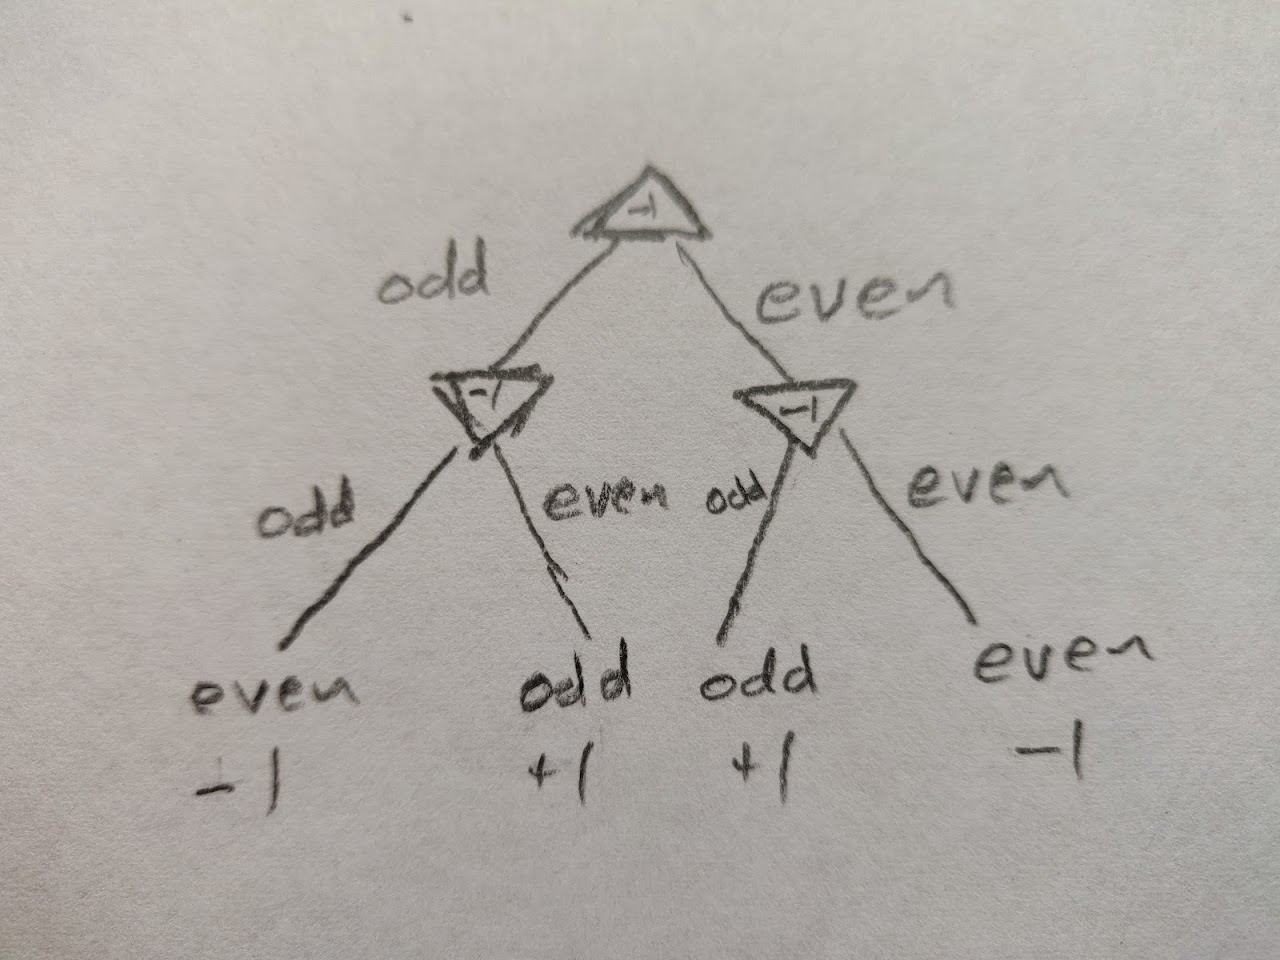
\includegraphics[width=0.3\textwidth]{odd-even-tree.jpg}
    
    Since we have assigned +1 to a win for Player 1 and -1 to a win for Player 2, and the value at the root node is -1, Player 2 will always win in optimal play.
\end{answer}

\begin{question}
    Consider a game where two people walking in opposite directions have to pass each other in a hallway:

\begin{tabular}{cc}
& Player 2 \\
    Player 1 &
    \begin{tabular}{c|c|c|}
          & L & R \\\hline
        L & -1,-1 & 1, 1 \\ \hline
        R & 1, 1 & -1,-1 \\ \hline
    \end{tabular}
\end{tabular}

\begin{enumerate}
    \item Describe the two pure strategy Nash equilibria and the value obtained by these.
    \item What is the value of the mixed-strategy Nash equilibrium where both players choose left or right with equal probability?
    \item Describe a correlated equilibrium where both players choose left and right with equal probability.
    \item Is it possible to find a correlated equilibrium where both players choose left and right with equal probability with a payoff equal to the pure strategy Nash equilibria?
\end{enumerate}

\end{question}

\begin{answer}
    \begin{enumerate}
        \item Either of the two strategies where players always play the opposite of each other are pure Nash equilibria (with a payoff of (1,1)).
        \item There is a 50\% chance that the players play the same direction, which yields a payoff of (-1,-1) and a 50\% chance that they play opposite, which yields a payoff of (1, 1), so the average payoff is (0,0).
        \item A coin that both players can see is flipped. If it is heads, player one chooses L and player two chooses R; if it is tails, player one chooses R and player two chooses L.
        \item Yes, the correlated equilibrium described above achieves a payoff of (1,1) since the players always play opposite actions.
    \end{enumerate} 
\end{answer}

\end{document}
